\section{Brainf*ck}\label{sec:brainfck}
\subsection{Language Description}
Brainf*ck is a popular esoteric programming language. Just like any other programming language, it allows the programmer to write programs consisting of commands that are executed in order. The key limitation is that the language provides only eight single-character commands to the programmer, all written as a single character: ``\texttt{+-<>[].,}''. Each of these commands corresponds to an operation on an array of memory or a pointer, pointing to some location within this memory. At the start of the program, every cell in (an infinite amount of) memory is initialized to 0 and the pointer is pointing to the very first element (index 0, see Figure \ref{fig:bfmachine_initial}).
%
\begin{figure}[H]
  \centering
  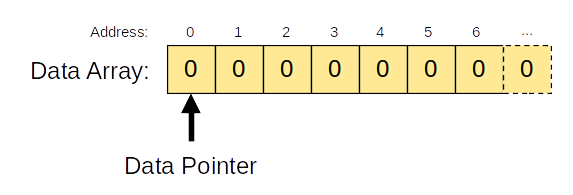
\includegraphics[width=0.5\textwidth]{img/bfmachine_initial}
  \caption{Initial state of the BF machine.}
  \label{fig:bfmachine_initial}
\end{figure}
%
The commands then modify the contents of memory and the pointer as follows:
\begin{itemize}
\item \texttt{+} : add 1 to the current cell;
\item \texttt{-} : subtract 1 from the current cell;
\item \texttt{<} : move the pointer 1 cell to its left;
\item \texttt{>} : move the pointer 1 cell to its right;
\item \texttt{[} : if the current cell is nonzero, continue. Otherwise, skip to the matching closing \texttt{]};
\item \texttt{]} : if the current cell is zero, continue. Otherwise, loop back to its matching opening \texttt{[};
\item \texttt{.} : send the value in the current cell to the output;
\item \texttt{,} : read a value from the input and store it into the current cell.
\end{itemize}
Although the instruction set is minimal, it has been proven to be sufficient for performing any possible computation or program, also known as Turing-completeness \cite{esolang}. The catch is that this requires an unbounded (or infinite) amount of memory, which is obviously impossible. However, the same caveat holds for traditional (von Neumann architecture) systems, so we should be safe to assume that BF is Turing complete for all practical purposes.

To run a BF program, one usually feeds these commands into an interpreter written in a more common language. These interpreters are very straightforward to write. Listing \ref{lst:bfint} shows a very simple implementation (about 40 lines) of such a program in C. This implementation initializes a block of memory to zero and defines a pointer to its first element. This pointer can be incremented or decremented to move along the array, increment/decrement value it's pointing or print it to standard output. The most complexity is embedded in the handling of the loop-operatores. When an opening bracket is encountered, the index of this instruction is stored in a jump-table. When the matching closing bracket is encountered and it is determined that flow should loop back, this stored index is reloaded. When a loop is being skipped, all commands within it are being skipped until the matching closing brace is found.

When the Hello World program from Wikipedia \cite{bfwiki} is fed into this program, it prints out the string \texttt{Hello World!}, as expected.
\begin{lstlisting}
  $ ./bfint "++++++++[>++++[>++>+++>+++>+<<<<-]>+>+>->>+[<]<-] \
  >>.>---.+++++++..+++.>>.<-.<.+++.------.--------.>>+.>++."
Hello World!
\end{lstlisting}


\begin{lstfloat}[H]
  \lstinputlisting[linerange={bfint\_begin-bfint\_end}, language=C]{../src/simple_int/bfint.c}  
\caption{Very basic implementation of a BF interpreter in C.}
\label{lst:bfint}
\end{lstfloat}



\subsection{Brainf*ck Architecture}
\paragraph{Von Neumann.} Modern computers are built according to the von Neumann architecture \cite{vonneumann-wiki}, which specifies a CPU (containing registers and an ALU), a single unit of memory and input/output devices (Figure \ref{fig:vonneumann}). The registers of the CPU can be loaded with data from the memory unit and operated on by the ALU (Arithmetic and Logic Unit). Typical about this kind of architecture is the fact that not only data, but also the instructions (the program) are stored in memory. The program is therefore just as much part of the data as the data itself and can even be modified by itself.
\begin{figure}[H]
  \centering
  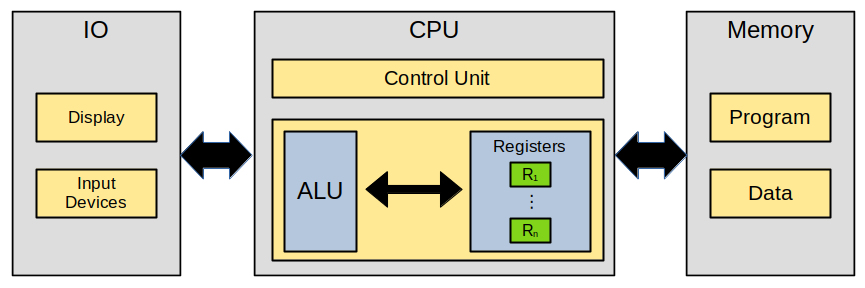
\includegraphics[width=0.9\textwidth]{img/vonneumann}
  \caption{Schematic overview of the Von Neumann architecture.}
  \label{fig:vonneumann}
\end{figure}

\paragraph{Harvard.} Unlike within the Von Neumann architecture, the Harvard architecture specifies two kinds of memory: program memory and data memory (Figure \ref{fig:harvard}). The program memory contains only the instructions to be carried out and cannot be modified at runtime. Other than that, the architecture is similar to Von Neumann, in that it consists of a CPU (again containing registers and an ALU), memory (program and data) and input/output devices.
\begin{figure}[H]
  \centering
  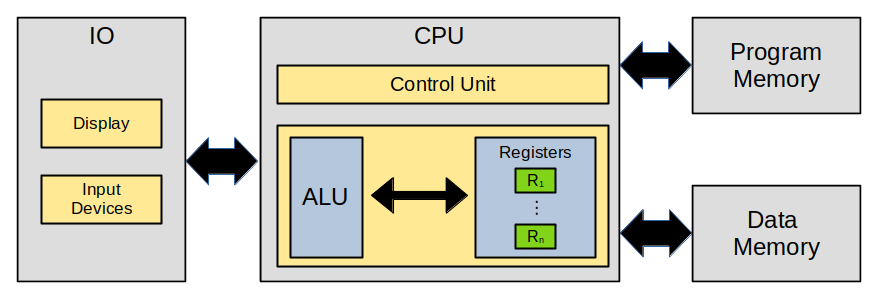
\includegraphics[width=0.9\textwidth]{img/harvard}
  \caption{Schematic overview of the Harvard architecture.}
  \label{fig:harvard}
\end{figure}

The architecture assumed by the BF language is similar to the Harvard architecture, in that the memory does not contain the program itself. This implies that the program is stored somewhere else and cannot be addressed by the pointer, like in Listing \ref{lst:bfint}, where the program was stored in a separate array to the data. The ALU is very limited and can only perform increment, decrement and comparison to zero.


\subsection{BF Instruction Set}
Instead of viewing BF as a language that needs to be compiled or interpreted on a traditional machine, it can also be seen as an instruction set to a processor, built according to the BF architecture described above. An instruction set of size 8 is truly tiny compared to more traditional instruction sets such as those implemented by modern processors or even microcontrollers and older 8-bit systems. Broadly speaking, Complex Instruction Set Computers (CISC) are designed to do as much work as possible in the least number of clock cycles, whereas Reduced Instruction Set Computers (RISC) focus on having a small instruction set with basic operations. For comparison, the x86 instruction set is massive with over 1500 instructions implemented in hardware, whereas RISC processors only need to implement 50 to 100 instructions. Even compared to RISC, the BF instruction set is tiny even compared to the smallest instruction sets in use today. This isn't necessarily a good thing; a smaller number of instructions simply means you need more of them to perform meaningful computations, which is reflected by the fact that complex BF programs are typically very large in size.

